% !TeX root = ../main.tex
\chapter{Unidad 8: Enfermedades auditivas, estudios diagnósticos y técnicas de rehabilitación}
\section*{Objetivo pedagógico}
\noindent\textbf{Objetivo.} Identificar las principales patologías auditivas (como tinnitus, presbiacusia y NIHL), comprender las pruebas diagnósticas (audiometría, OEA, PEA) y evaluar las opciones de rehabilitación tecnológica (audífonos, implantes cocleares) según el tipo y grado de pérdida auditiva, aplicando estos conocimientos en la práctica fonoaudiológica. Se incluyen ejemplos clínicos, actividades prácticas, recursos multimedia y ejercicios de autoevaluación.

\noindent\textbf{Pregunta inicial.} ¿Cómo se detecta una pérdida auditiva? ¿Qué opciones existen para ayudar a un paciente a escuchar mejor? ¡Esta unidad te ayudará a entender cómo diagnosticar y tratar problemas auditivos!

\section{Fatiga auditiva y daño inducido por ruido}

\subsection{Desplazamiento temporal del umbral (TTS)}
La exposición breve a ruidos fuertes ($>$85 dBSPL, como un concierto) eleva temporalmente el umbral de audición (TTS). La recuperación suele tomar 2–48 horas.

\begin{itemize}
    \item \textbf{Mecanismo:} Las células ciliadas externas (CCE) se agotan metabólicamente, causando edemas celulares.
    \item \textbf{Relevancia clínica:} TTS repetidos (por ejemplo, escuchar música alta frecuentemente) pueden llevar a daño permanente.
\end{itemize}

\begin{quote}
    \textbf{Ejemplo clínico.} Un adolescente que usa auriculares a 90 dB durante horas puede experimentar zumbidos temporales (TTS), un signo de alerta para prevenir daño permanente.
\end{quote}

\subsection{Pérdida auditiva inducida por ruido (NIHL)}
El \textbf{NIHL} (Noise-Induced Hearing Loss) es un daño permanente a las CCE, con un “notch” característico en 3–6 kHz en el audiograma. El riesgo depende del nivel equivalente ($L_{Aeq,8h}$) y los años de exposición.

\begin{quote}
    \textbf{Ejemplo clínico.} Un trabajador de fábrica expuesto a 90 dBA durante 20 años puede desarrollar un notch en 4 kHz, dificultando la comprensión de consonantes como ``s'' o ``f''.
\end{quote}

\paragraph{Normativa} La exposición laboral debe ser $<$85 dBA durante 8 horas (según OMS y normativas locales). Se usan protectores auditivos (NRR, Noise Reduction Rating) para reducir el riesgo.

\textbf{Actividad práctica.} Usa una app como Decibel X (gratis) para medir el nivel de ruido en un entorno ruidoso (como un café o concierto). Si supera 85 dBA, calcula cuánto tiempo es seguro permanecer sin protección.

\section{Trauma acústico y ototóxicos}
Un \textbf{trauma acústico} ($>$140 dBSPL, como una explosión) puede perforar el tímpano o dañar la membrana basilar. El tratamiento inmediato con corticosteroides puede minimizar la pérdida.

\begin{itemize}
    \item \textbf{Ototóxicos:} Fármacos como aminoglucósidos (gentamicina) o cisplatino dañan las CCE. Se monitorean con otoemisiones acústicas (OEA) y audiometría en altas frecuencias ($>$8 kHz).
\end{itemize}

\begin{quote}
    \textbf{Ejemplo clínico.} Un paciente en quimioterapia con cisplatino necesita pruebas regulares de OEA para detectar daño coclear temprano y ajustar el tratamiento.
\end{quote}

\section{Tinnitus y presbiacusia}

\subsection{Tinnitus}
El \textbf{tinnitus} es la percepción de zumbidos o sonidos sin fuente externa (prevalencia: 10–15\%). Se asocia con plasticidad cortical tras daño auditivo.

\begin{description}
    \item[\textbf{Enmascaramiento:}] Ruido de banda ancha a 5–10 dB sobre el tinnitus reduce su percepción.
    \item[\textbf{TRT (Tinnitus Retraining Therapy):}] Combina consejería y ruido modulador para habituar al paciente al tinnitus.
\end{description}

\begin{quote}
    \textbf{Ejemplo clínico.} Un paciente con tinnitus a 4 kHz puede usar un audífono con ruido de enmascaramiento para aliviar la molestia durante el día.
\end{quote}

\subsection{Presbiacusia}
La \textbf{presbiacusia} es la pérdida auditiva relacionada con la edad, con una pendiente de más de 2 dB por década en frecuencias mayores a 2 kHz. Afecta la inteligibilidad del habla, especialmente en agudos.

\begin{quote}
    \textbf{Ejemplo clínico.} Un adulto mayor con presbiacusia necesita audífonos que amplifiquen frecuencias altas (2–8 kHz) sin retroalimentación, mejorando la comprensión de palabras.
\end{quote}

\begin{figure}[h]
    \centering
    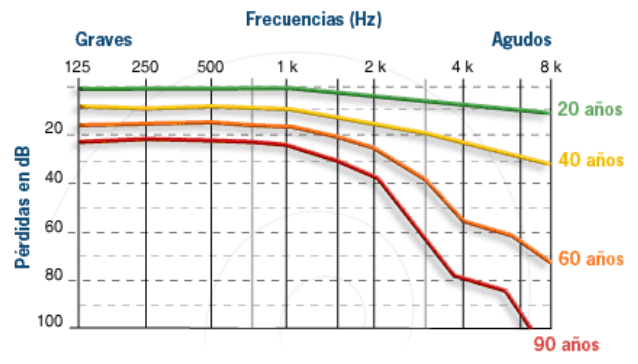
\includegraphics[width=0.9\textwidth]{figures/presbiacusia.png}
    \caption{Evolución de la presbiacusia con los años.}
    \label{fig:presbiacusia}
\end{figure}

\section{Estudios de la audición}

\subsection{Audiometría tonal}
Mide los umbrales de audición vía aérea y ósea (250 Hz–8 kHz). Clasificación de la pérdida:
\begin{itemize}
    \item Leve: 26–40 dB HL
    \item Moderada: 41–55 dB HL
    \item Moderada-severa: 56–70 dB HL
    \item Severa: 71–90 dB HL
    \item Profunda: $>$90 dB HL
\end{itemize}

\begin{quote}
    \textbf{Ejemplo clínico.} Un paciente con umbrales de 50 dB HL a 4 kHz (vía aérea) y 20 dB HL (vía ósea) tiene hipoacusia conductiva, posiblemente por otosclerosis.
\end{quote}

\subsection{Logoaudiometría}
Estudio que evalúa el reconocimiento de palabras (\%). La curva PI-PB (Phonetically Balanced) muestra el porcentaje de palabras entendidas según el nivel (dBSPL). Un “roll-over” (caída a niveles altos) indica lesión retrococlear.

\subsection{Timpanometría}
Mide la presión y compliancia del oído medio. Tipos:
\begin{itemize}
    \item \textbf{Tipo A:} Normal (pico de presión).
    \item \textbf{Tipo B:} Sin pico (otitis media serosa).
    \item \textbf{Tipo C:} Pico desplazado (disfunción de trompa de Eustaquio).
\end{itemize}

\begin{figure}[h]
    \centering
    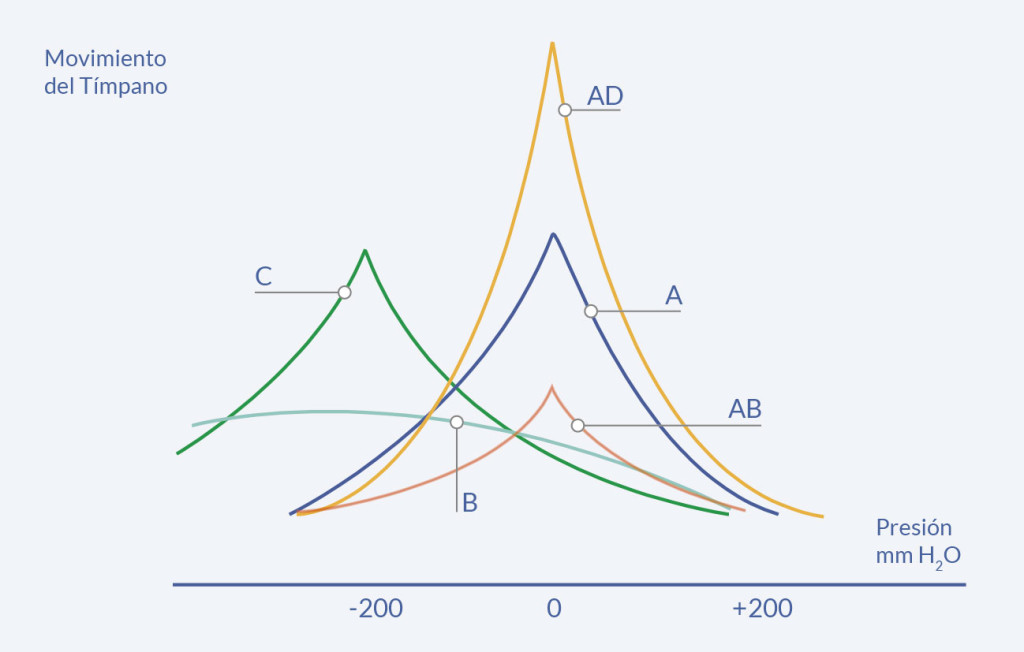
\includegraphics[width=0.9\textwidth]{figures/timpanometria.png}
    \caption{Tipos de resultados de timpanometrías.}
    \label{fig:timpanometria}
\end{figure}

\subsection{Acufenometría}
Compara el pitch y la intensidad del tinnitus con tonos puros para diseñar terapias de enmascaramiento.

\subsection{Pruebas electrofisiológicas}
\begin{itemize}
    \item \textbf{OEA (Otoemisiones Acústicas):} Evalúa las CCE. Usada en screening neonatal (dura $\approx$2 min).
    \item \textbf{PEA (Auditory Brainstem Response):} Mide latencias de ondas I–V ($<$10 ms) para evaluar la vía neural.
    \item \textbf{ECochG (Electrocochleografía):} Registra potenciales cocleares (SP, AP), útil en la enfermedad de Ménière.
\end{itemize}

\begin{table}[h]
    \centering
    \begin{tabular}{|l|c|c|c|}
        \hline
        \textbf{Prueba} & \textbf{Duración} & \textbf{Invasiva} & \textbf{Evalúa} \\
        \hline
        Audiometría & 10 min & No & Umbrales (conductiva/sensorial) \\
        OEA & 2 min & No & Función de CCE \\
        PEA & 15 min & No & Vía neural/retrococlear \\
        ECochG & 30 min & Sí* & Potenciales cocleares \\
        \hline
    \end{tabular}
    \caption{Comparación de estudios auditivos (*vía tímpano, requiere médico).}
\end{table}

\begin{quote}
    \textbf{Ejemplo clínico.} Un neonato con OEA ausente puede tener hipoacusia sensorioneural, confirmada con PEA para evaluar el nervio auditivo.
\end{quote}

\section{Rehabilitación tecnológica}

\subsection{Audífonos}
Amplifican sonidos con tecnología WDRC (Wide Dynamic Range Compression), hasta 70 dB de ganancia. Incluyen:
\begin{itemize}
    \item Micrófonos direccionales para mejorar la SNR.
    \item Cancelación de feedback (retroalimentación).
    \item Conectividad Bluetooth para teléfonos.
\end{itemize}

\begin{quote}
    \textbf{Ejemplo clínico.} Un paciente con presbiacusia usa un audífono que amplifica 2–8 kHz, con micrófonos direccionales para mejorar la inteligibilidad en entornos ruidosos.
\end{quote}

\subsection{Implante coclear (IC)}
Indicado para hipoacusia severa-profunda ($<$50\% reconocimiento de palabras). Usa 12–24 electrodos para estimular el nervio auditivo según el mapa tonotópico.

\subsection{Implantes osteointegrados (BAHA)}
Vibran la mastoides para hipoacusia conductiva (por ejemplo, atresia del CAE o infecciones crónicas).

\subsection{EAS (Electro-Acoustic Stimulation)}
Combina amplificación acústica ($<$1 kHz) con estimulación eléctrica ($>$1 kHz) para pacientes con audición residual en graves.


\section{Ejemplos prácticos}
\begin{enumerate}
    \item \textbf{Clasificación de pérdida.} Un paciente con un notch de 40 dB a 4 kHz y umbrales normales en 1 kHz tiene hipoacusia leve sensorioneural (NIHL). Consejería: usar protectores auditivos y monitorear anualmente.
    \item \textbf{Cálculo de $L_{Aeq,8h}$.} 95 dBA durante 1 h equivale a:
    \[
    L_{Aeq,8h} = 95 - 10 \log_{10}\left(\frac{8}{1}\right) \approx 86 \, \text{dBA}.
    \]
    \item \textbf{Ganancia necesaria.} Para un umbral de 60 dB a 2 kHz, la regla half-gain sugiere:
    \[
    \text{Ganancia} = \frac{60 - 20}{2} = 20 \, \text{dB}.
    \]
\end{enumerate}

\section{Ejercicios de autoevaluación}
\begin{enumerate}
    \item Compara el “notch” de NIHL con la pendiente de presbiacusia en un audiograma. ¿Cómo afecta cada uno a la inteligibilidad del habla?
    \item Describe los pasos de una prueba PEA y explica qué indica un retraso en la onda III.
    \item Enumera ventajas (mejor audición, conectividad) y limitaciones (costo, cirugía) del implante coclear en mayores de 70 años.
    \item Usa Decibel X para medir el ruido en un entorno (por ejemplo, un aula). Si supera 85 dBA, sugiere medidas preventivas.
\end{enumerate}

\section{Recursos recomendados}
\begin{itemize}
    \item Video: \href{https://www.youtube.com/watch?v=PnmRgyi4-dU&ab_channel=Cl%C3%ADnicaUniversidaddeNavarra}{``Implantes cocleares | Qué son, cómo funcionan y qué pacientes son candidatos''}.
    \item App: Tinnitus Relief (gratis). Ofrece sonidos para TRT.
    \item App: Decibel X (gratis). Mide niveles de ruido.
    \item Documento: OMS, \emph{Make Listening Safe} (PDF disponible en línea).
    \item Libro: J. Katz, \emph{Handbook of Clinical Audiology}, capítulos 10–12.
\end{itemize}

\section*{Glosario}
\begin{description}
    \item[\textbf{TTS:}] Desplazamiento temporal del umbral, reversible.
    \item[\textbf{NIHL:}] Pérdida auditiva inducida por ruido, con notch en 3–6 kHz.
    \item[\textbf{TRT:}] Terapia de reentrenamiento para tinnitus.
    \item[\textbf{PEA:}] Respuesta auditiva del tronco encefálico, mide latencias neurales.
    \item[\textbf{BAHA:}] Audífono anclado al hueso, para hipoacusia conductiva.
\end{description}

\section*{Resumen}
\begin{itemize}
    \item \textbf{Patologías:} NIHL (notch 3–6 kHz), presbiacusia (pendiente $>$2 kHz), tinnitus (zumbidos).
    \item \textbf{Diagnósticos:} Audiometría (umbrales), OEA (CCE), PEA (vía neural).
    \item \textbf{Rehabilitación:} Audífonos (WDRC), implantes cocleares (severa-profunda), BAHA/EAS.
\end{itemize}


\bigskip
\noindent\emph{Conclusión.} Comprender las patologías auditivas, las pruebas diagnósticas y las tecnologías de rehabilitación permite diseñar intervenciones personalizadas, mejorando la calidad de vida de los pacientes.



%%%%%%%%%%%%%%%%%%%%%%%%%%%%%%%%%%%%%%%%%%%%%%%%%%%%%%%%%%%%%%%%%%%%%%%%%%%%%%%%%%%%%%%%%%%%%%%%%%
